\documentclass[a4paper,14pt]{extarticle}
%\documentclass[a4paper]{article}
\usepackage[T2A]{fontenc}
\usepackage[utf8]{inputenc}
\usepackage[english,russian]{babel}
\usepackage{indentfirst}
\usepackage{amssymb}
\usepackage{amsfonts}
\usepackage{amsmath}
\usepackage{mathtext}
\usepackage{cite}
\usepackage{enumerate}
\usepackage{hyphenat}
\usepackage{float}
\usepackage[top=1.5cm,bottom=1.5cm,left=2.5cm,right=1.5cm]{geometry}
\usepackage[unicode]{hyperref}
\usepackage{graphicx}
\usepackage{color}
\usepackage[colorinlistoftodos]{todonotes}
\usepackage[format=hang, labelsep=period, margin=10pt, figurename=Рис.]{caption}
\usepackage{listings}
\usepackage{subcaption}
%\usepackage{showkeys}
\usepackage[onehalfspacing]{setspace}



\definecolor{dkgreen}{rgb}{0,0.6,0}
\definecolor{gray}{rgb}{0.5,0.5,0.5}
\definecolor{mauve}{rgb}{0.58,0,0.82}
 
\lstset{ %
  language=C++,                % the language of the code
  basicstyle=\footnotesize,           % the size of the fonts that are used for the code
%  numbers=left,                   % where to put the line-numbers
%  numberstyle=\tiny\color{gray},  % the style that is used for the line-numbers
%  stepnumber=2,                   % the step between two line-numbers. If it's 1, each line 
                                  % will be numbered
  numbersep=5pt,                  % how far the line-numbers are from the code
  backgroundcolor=\color{white},      % choose the background color. You must add \usepackage{color}
  showspaces=false,               % show spaces adding particular underscores
  showstringspaces=false,         % underline spaces within strings
  showtabs=false,                 % show tabs within strings adding particular underscores
  frame=single,                   % adds a frame around the code
  rulecolor=\color{black},        % if not set, the frame-color may be changed on line-breaks within not-black text (e.g. commens (green here))
  tabsize=2,                      % sets default tabsize to 2 spaces
  captionpos=b,                   % sets the caption-position to bottom
  breaklines=true,                % sets automatic line breaking
  breakatwhitespace=false,        % sets if automatic breaks should only happen at whitespace
  title=\lstname,                   % show the filename of files included with \lstinputlisting;
                                  % also try caption instead of title
  keywordstyle=\color{blue},          % keyword style
  commentstyle=\color{dkgreen},       % comment style
  stringstyle=\color{mauve},         % string literal style
  escapeinside={\%*}{*)},            % if you want to add a comment within your code
  morekeywords={*,...}               % if you want to add more keywords to the set
}
\renewcommand\lstlistingname{Листинг}
\renewcommand\lstlistlistingname{Листинги}
\newcommand{\itodo}{\todo[inline]}
\lstloadlanguages{C++}
\DeclareCaptionFont{blue}{\color{blue}} 
%\%captionsetup[lstlisting]{singlelinecheck=false, labelfont={blue}, textfont={blue}}
%\DeclareCaptionFont{white}{\color{white}}
%\DeclareCaptionFormat{listing}{\colorbox[cmyk]{0.43, 0.35, 0.35,0.01}{\parbox{\textwidth}{\hspace{15pt}#1#2#3}}}
%\captionsetup[lstlisting]{
%	format=listing,
%	labelfont=white,
%	textfont=white,
%	singlelinecheck=false,
%	margin=0pt,
%	font={bf,footnotesize}
%}
\numberwithin{equation}{section}
\setcounter{secnumdepth}{3} % глубина нумеруемых разделов
\setcounter{tocdepth}{3} % глубина оглавления
\begin{document}
%\listoftodos
%\clearpage
\newpage
\begin{titlepage}
\newpage

\begin{center}
	Министерство образования и науки Российской Федерации \\
	МОСКОВСКИЙ ФИЗИКО-ТЕХНИЧЕСКИЙ ИНСТИТУТ\\(государственный университет)\\[0.5cm]
	ФАКУЛЬТЕТ АЭРОФИЗИКИ И КОСМИЧЕСКИХ ИССЛЕДОВАНИЙ\\
	КАФЕДРА ВЫЧИСЛИТЕЛЬНОЙ МАТЕМАТИКИ\\
	(Специализация «Компьютерное моделирование\\
	в механике, биомеханике и физиологии»)\\[1cm]
\end{center}

\vspace{1em}

\begin{center}
	\textsc{\textbf{Численное моделирование\\
	 сеточно-характеристическим методом\\
	 волновых процессов при неразрушающем контроле\\
	 изделий из изотропных и анизотропных\\
	 композитных материалов}}\\[2cm]
	Магистерская диссертация\\[0.5cm]
	студента 031 группы\\
	Казакова Александра Олеговича\\
\end{center}

\vspace{1.5em}

\begin{center}
	Научный руководитель\\
	Васюков Алексей Викторович, к.ф.-м.н.
\end{center}

%\vspace{3.5em}
\vfill

\begin{center}
	г.Долгопрудный\\
	2016
\end{center}


\end{titlepage}

\tableofcontents
\clearpage
\newpage
\section*{Введение}
\addcontentsline{toc}{section}{Введение}
В данной работе рассматривается численное моделирование волновых деформационных процессов в твёрдых телах. Для описание физических процессов используются уравнения на скорости и напряжения в частицах материала из механики сплошной среды для деформируемого твёрдого тела. Рассчёт имеющейся системы уравнений проводится численно сеточно-характеристическим методом с расщеплением по трём пространственным направлениям. Он позволяет получать динамическую волновую картину.


\begin{itemize}
\item а
\item б
\item в
\item г
\end{itemize}

\clearpage
\newpage
\section{Обзор существующих работ по данной тематике}

Комбинация математической модели линейно-упругого тела и сеточно-характеристического численного метода для расчёта волновых задач используется уже давно и хорошо себя зарекомендовала.

Сеточно\hyp{}характеристический метод численного решения уравнений в частных производных гиперболического типа был впервые предложен в \cite{magomedov_kholodov_1969}. В последствии его авторами была выпущена подробная монография по различным аспектам его применения и реализации \cite{magomedov_kholodov_1988}.

Одно из первых применений метода к расчёту волновых задач механики деформируемого твёрдого тела было осуществлено в \cite{petrov_kholodov} на структурированных расчётных сетках. Возможность применения метода с высоким порядком аппроксимации на неструктурированных расчётных сетках была продемонстрирована в работе \cite{chelnokov_agapov}. Значительные улучшения метода, связанные со спектральным разложением матриц системы уравнений и расчётом граничных и контактных узлов, были предложены в \cite{chelnokov}. В работе \cite{favorskaya_anysotropy} был предложен способ диагонализации матриц системы уравнений для произвольного случая анизотропии материала. Реализация метода на  структурированных иерархических тетраэдральных сетках с кратным шагом по времени продемонстрирована в работе \cite{favorskaya}.

В монографии \cite{kulikovskiy} рассмотрены различные математические вопросы сеточно\hyp{}характеристического метода и других родственных ему методов численного решения динамических волновых задач.

Таким образом, данная область знаний уже является хорошо изученной, однако полная реализация всех методов в трёхмерном пространстве с различной реологией материалов, сложной геометрией областей и другими практическими аспектами, важными в прикладных задачах, всё ещё оставляет много вопросов.
\clearpage
\newpage
\section{Уравнения механики линейно-упругого тела}

\subsection{Общий вид уравнений}
\label{model}

Для математического моделирования волновых процессов в деформируемом твёрдом
теле используется система динамических уравнений \cite{sedov, kukudzhanov} в виде
\begin{eqnarray}
	\label{initial_equations}
	\rho\dot{v}_i=\nabla_j\sigma_{ij}+f_i & \textrm{(уравнения движения)}\nonumber\\
	\dot{\sigma}_{ij}=q_{ijkl}\dot{\varepsilon}_{kl}+F_{ij} & \textrm{(реологические соотношения).}
\end{eqnarray}

Здесь $\rho$ – плотность среды, $v_i$ – компоненты векторов скорости частиц среды,
$\sigma_{ij}$, $\varepsilon_{ij}$ -- компоненты симметричных тензоров напряжений и деформаций,
$\nabla_j$ – производная по $j$-й координате, $f_i$ – массовые
силы, действующие на единицу объёма, $F_{ij}$ -- силы, обусловленные вязкостью, $q_{ijkl}$ -- 
тензор упругих постоянных.

В случае малых деформаций тензор скоростей деформаций $e_{ij}=\dot{\varepsilon}_{ij}$ 
выражается через компоненты скорости смещения линейным образом:
\begin{equation}
	e_{ij}=\frac{1}{2}(\nabla_j v_i+\nabla_i v_j).
\end{equation}

Компоненты тензора 4-го порядка $q_{ijkl}$, сил вязкости $F_{ij}$ и плотности $\rho$ определяются реологией среды. 

\subsection{Случай изотропного линейно-упругого тела}
Для невязкого изотропного линейно-упругого материала
\begin{eqnarray}
	\label{isotropic_tensor}
	q_{ijkl}=\lambda\delta_{ij}\delta_{kl}+\mu(\delta_{ik}\delta_{jl}+\delta_{il}
	\delta_{jk}) & \textrm {(изотропия)} \nonumber\\
	F_{ij}=0 & \textrm {(отсутствует вязкость)} \\
	\rho=const & \textrm {(изменения пренебрежимо малы)}.
\end{eqnarray}

В этом соотношении, которое обобщает закон Гука, $\lambda$ и $\mu$ -- параметры
Ляме, связанные с более известными модулем Юнга $E$ и коэффициентом Пуассона $\nu$ (модулем сдвига $G$) следующими соотношениями:
\begin{eqnarray}
\label{lame_parameters}
	\lambda &= \frac{E\nu}{(1+\nu)(1-2\nu)}
	\nonumber\\
	\mu &= G=\frac{E}{2(1+\nu)}.
\end{eqnarray}


В этом случае уравнения \eqref{initial_equations} принимают вид:
\begin{align}
	\label{simple_equations}
	\frac{\partial{v_x}}{\partial{t}}&=\frac{1}{\rho}(\frac{\partial{\sigma_{xx}}}{\partial{x}}+\frac{\partial{\sigma_{xy}}}{\partial{y}}+\frac{\partial{\sigma_{xz}}}{\partial{z}})
	\nonumber\\
	\frac{\partial{v_y}}{\partial{t}}&=\frac{1}{\rho}(\frac{\partial{\sigma_{xy}}}{\partial{x}}+\frac{\partial{\sigma_{yy}}}{\partial{y}}+\frac{\partial{\sigma_{yz}}}{\partial{z}})
	\nonumber\\
	\frac{\partial{v_z}}{\partial{t}}&=\frac{1}{\rho}(\frac{\partial{\sigma_{xz}}}{\partial{x}}+\frac{\partial{\sigma_{yz}}}{\partial{y}}+\frac{\partial{\sigma_{zz}}}{\partial{z}})
	\nonumber\\
	\frac{\partial{\sigma_{xx}}}{\partial{t}}&=(\lambda+2\mu)\frac{\partial{v_x}}{\partial{x}}+\lambda\frac{\partial{v_y}}{\partial{y}}+\lambda\frac{\partial{v_z}}{\partial{z}}
	\nonumber\\
	\frac{\partial{\sigma_{xy}}}{\partial{t}}&=\mu(\frac{\partial{v_x}}{\partial{y}}+\frac{\partial{v_y}}{\partial{x}})
	\nonumber\\
	\frac{\partial{\sigma_{xz}}}{\partial{t}}&=\mu(\frac{\partial{v_x}}{\partial{z}}+\frac{\partial{v_z}}{\partial{x}})
	\nonumber\\
	\frac{\partial{\sigma_{yy}}}{\partial{t}}&=\lambda\frac{\partial{v_x}}{\partial{x}}+(\lambda+2\mu)\frac{\partial{v_y}}{\partial{y}}+\lambda\frac{\partial{v_z}}{\partial{z}}
	\nonumber\\
	\frac{\partial{\sigma_{yz}}}{\partial{t}}&=\mu(\frac{\partial{v_z}}{\partial{y}}+\frac{\partial{v_y}}{\partial{z}})
	\nonumber\\
	\frac{\partial{\sigma_{zz}}}{\partial{t}}&=\lambda\frac{\partial{v_x}}{\partial{x}}+\lambda\frac{\partial{v_y}}{\partial{y}}+(\lambda+2\mu)\frac{\partial{v_z}}{\partial{z}}
\end{align}

Обозначив искомый вектор $\vec{u}=\{v_x,v_y,v_z,\sigma_{xx},\sigma_{xy},\sigma_{xz},\sigma_{yy},\sigma_{yz},\sigma_{zz}\}^T$, уравнения \eqref{initial_equations} можно переписать в матричной форме \cite{petrov_kholodov}:

\begin{equation}
	\label{simple_matrix_equation}
	\frac{\partial\vec{u}}{\partial{t}}+\mathbf{A}_x\frac{\partial\vec{u}}{\partial{x}}+
	\mathbf{A}_y\frac{\partial\vec{u}}{\partial{y}}+
	\mathbf{A}_z\frac{\partial\vec{u}}{\partial{z}}=0,
\end{equation}
где матрицы $\mathbf{A}_x$, $\mathbf{A}_y$, $\mathbf{A}_z$ принимают следующий вид:

\begin{align}
\label{isotropic_mat1}
\mathbf{A}_x =
\left( \begin{array}{cccccccccccc}
0 & 0 & 0 & -\frac 1 \rho & 0 & 0 & 0 & 0 & 0 \\ 
0 & 0 & 0 & 0 & -\frac 1 \rho & 0 & 0 & 0 & 0 \\ 
0 & 0 & 0 & 0 & 0 & -\frac 1 \rho & 0 & 0 & 0 \\ 
-(\lambda+2\mu) & 0 & 0 & 0 & 0 & 0 & 0 & 0 & 0 \\ 
0 & -\mu & 0 & 0 & 0 & 0 & 0 & 0 & 0 \\ 
0 & 0 & -\mu & 0 & 0 & 0 & 0 & 0 & 0 \\ 
-\lambda & 0 & 0 & 0 & 0 & 0 & 0 & 0 & 0 \\ 
0 & 0 & 0 & 0 & 0 & 0 & 0 & 0 & 0 \\ 
-\lambda & 0 & 0 & 0 & 0 & 0 & 0 & 0 & 0  
\end{array} \right),
\end{align} 
\begin{align}
\label{isotropic_mat2}
\mathbf{A}_y =
\left( \begin{array}{cccccccccccc}
0 & 0 & 0 & 0 & -\frac 1 \rho & 0 & 0 & 0 & 0 \\ 
0 & 0 & 0 & 0 & 0 & 0 & -\frac 1 \rho & 0 & 0 \\ 
0 & 0 & 0 & 0 & 0 & 0 & 0 & -\frac 1 \rho & 0 \\ 
0 & -\lambda & 0 & 0 & 0 & 0 & 0 & 0 & 0 \\ 
-\mu & 0 & 0 & 0 & 0 & 0 & 0 & 0 & 0 \\ 
0 & 0 & 0 & 0 & 0 & 0 & 0 & 0 & 0 \\ 
0 & -(\lambda+2\mu) & 0 & 0 & 0 & 0 & 0 & 0 & 0 \\ 
0 & 0 & -\mu & 0 & 0 & 0 & 0 & 0 & 0 \\ 
0 & -\lambda & 0 & 0 & 0 & 0 & 0 & 0 & 0  
\end{array} \right),
\end{align}
\begin{align}
\label{isotropic_mat3}
\mathbf{A}_z =
\left( \begin{array}{cccccccccccc}
0 & 0 & 0 & 0 & 0 & -\frac 1 \rho & 0 & 0 & 0 \\ 
0 & 0 & 0 & 0 & 0 & 0 & 0 & -\frac 1 \rho & 0 \\ 
0 & 0 & 0 & 0 & 0 & 0 & 0 & 0 & -\frac 1 \rho \\ 
0 & 0 & -\lambda & 0 & 0 & 0 & 0 & 0 & 0 \\ 
0 & 0 & 0 & 0 & 0 & 0 & 0 & 0 & 0 \\ 
-\mu & 0 & 0 & 0 & 0 & 0 & 0 & 0 & 0 \\ 
0 & 0 & -\lambda & 0 & 0 & 0 & 0 & 0 & 0 \\ 
0 & -\mu & 0 & 0 & 0 & 0 & 0 & 0 & 0 \\ 
0 & 0 & -(\lambda+2\mu) & 0 & 0 & 0 & 0 & 0 & 0  
\end{array} \right).
\end{align}\\


\subsection{Случай произвольно анизотропного линейно-упругого тела}
Для материала с произвольным типом анизотропии тензор упругих постоянных $q_{ijkl}$ обладает 21 независимым параметром.
Это видно из следующих рассуждений \cite{prodaivoda}. Вообще говоря, число его компонент $3^4 = 81$. Однако симметричные в рассматриваемой модели тензоры напряжений и деформаций имеют не 9, а 6 независимых компонент. Остаётся 36 независимых компонент $q_{ijkl}$. Теперь рассмотрим выражение для потенциала упругой энергии $W$:

\begin{eqnarray}
dW &= \sigma_{ij} d\varepsilon_{ij}, \\
q_{ijkl} &= \frac{\partial{\sigma_{ij}}}{\partial{\varepsilon_{kl}}}, \\
q_{ijkl} &= \frac{\partial^{2}{W}}{\partial{\varepsilon_{ij}\varepsilon_{kl}}}.
\end{eqnarray}

Из независимости второй производной от порядка дифференцирования следует $q_{ijkl} = q_{klij}$. Теперь зависимость $\sigma$ от $\varepsilon$ можно записать в более компактном виде:
\begin{align}
\left( \begin{array}{cccccccccccc}
\sigma_{11} \\
\sigma_{22} \\
\sigma_{33} \\
\sigma_{23} \\
\sigma_{13} \\
\sigma_{12} 
\end{array} \right){}
= \left( \begin{array}{cccccccccccc}
c_{11} & c_{12} & c_{13} & c_{14} & c_{15} & c_{16} \\ 
c_{12} & c_{22} & c_{23} & c_{24} & c_{25} & c_{26} \\ 
c_{13} & c_{23} & c_{33} & c_{34} & c_{35} & c_{36} \\ 
c_{14} & c_{24} & c_{34} & c_{44} & c_{45} & c_{46} \\ 
c_{15} & c_{25} & c_{35} & c_{45} & c_{55} & c_{56} \\ 
c_{16} & c_{26} & c_{36} & c_{46} & c_{56} & c_{66}
\end{array} \right){}
\left( \begin{array}{cccccccccccc}
\varepsilon_{11} \\
\varepsilon_{22} \\
\varepsilon_{33} \\
\varepsilon_{23} \\
\varepsilon_{13} \\
\varepsilon_{12}
\end{array} \right)
\end{align}


Такми образом, для случая произвольной анизотропии уравнения \eqref{initial_equations} принимают вид:
\begin{small}
\begin{align}
	\label{anisotropic_equations}
	\frac{\partial{v_x}}{\partial{t}}&=\frac{1}{\rho}(\frac{\partial{\sigma_{xx}}}{\partial{x}}+\frac{\partial{\sigma_{xy}}}{\partial{y}}+\frac{\partial{\sigma_{xz}}}{\partial{z}})
	\nonumber\\
	\frac{\partial{v_y}}{\partial{t}}&=\frac{1}{\rho}(\frac{\partial{\sigma_{xy}}}{\partial{x}}+\frac{\partial{\sigma_{yy}}}{\partial{y}}+\frac{\partial{\sigma_{yz}}}{\partial{z}})
	\nonumber\\
	\frac{\partial{v_z}}{\partial{t}}&=\frac{1}{\rho}(\frac{\partial{\sigma_{xz}}}{\partial{x}}+\frac{\partial{\sigma_{yz}}}{\partial{y}}+\frac{\partial{\sigma_{zz}}}{\partial{z}})
	\nonumber\\
	\frac{\partial{\sigma_{xx}}}{\partial{t}}&=c_{11}\frac{\partial{v_x}}{\partial{x}}+c_{12}\frac{\partial{v_y}}{\partial{y}}+c_{13}\frac{\partial{v_z}}{\partial{z}}+c_{14}(\frac{\partial{v_z}}{\partial{y}}+\frac{\partial{v_y}}{\partial{z}})+c_{15}(\frac{\partial{v_z}}{\partial{x}}+\frac{\partial{v_x}}{\partial{z}})+c_{16}(\frac{\partial{v_y}}{\partial{x}}+\frac{\partial{v_x}}{\partial{y}})
	\nonumber\\
	\frac{\partial{\sigma_{yy}}}{\partial{t}}&=c_{12}\frac{\partial{v_x}}{\partial{x}}+c_{22}\frac{\partial{v_y}}{\partial{y}}+c_{23}\frac{\partial{v_z}}{\partial{z}}+c_{24}(\frac{\partial{v_z}}{\partial{y}}+\frac{\partial{v_y}}{\partial{z}})+c_{25}(\frac{\partial{v_z}}{\partial{x}}+\frac{\partial{v_x}}{\partial{z}})+c_{26}(\frac{\partial{v_y}}{\partial{x}}+\frac{\partial{v_x}}{\partial{y}})
	\nonumber\\
	\frac{\partial{\sigma_{zz}}}{\partial{t}}&=c_{13}\frac{\partial{v_x}}{\partial{x}}+c_{23}\frac{\partial{v_y}}{\partial{y}}+c_{33}\frac{\partial{v_z}}{\partial{z}}+c_{34}(\frac{\partial{v_z}}{\partial{y}}+\frac{\partial{v_y}}{\partial{z}})+c_{35}(\frac{\partial{v_z}}{\partial{x}}+\frac{\partial{v_x}}{\partial{z}})+c_{36}(\frac{\partial{v_y}}{\partial{x}}+\frac{\partial{v_x}}{\partial{y}})
	\nonumber\\
	\frac{\partial{\sigma_{yz}}}{\partial{t}}&=c_{14}\frac{\partial{v_x}}{\partial{x}}+c_{24}\frac{\partial{v_y}}{\partial{y}}+c_{34}\frac{\partial{v_z}}{\partial{z}}+c_{44}(\frac{\partial{v_z}}{\partial{y}}+\frac{\partial{v_y}}{\partial{z}})+c_{45}(\frac{\partial{v_z}}{\partial{x}}+\frac{\partial{v_x}}{\partial{z}})+c_{46}(\frac{\partial{v_y}}{\partial{x}}+\frac{\partial{v_x}}{\partial{y}})
	\nonumber\\
	\frac{\partial{\sigma_{xz}}}{\partial{t}}&=c_{15}\frac{\partial{v_x}}{\partial{x}}+c_{25}\frac{\partial{v_y}}{\partial{y}}+c_{35}\frac{\partial{v_z}}{\partial{z}}+c_{45}(\frac{\partial{v_z}}{\partial{y}}+\frac{\partial{v_y}}{\partial{z}})+c_{55}(\frac{\partial{v_z}}{\partial{x}}+\frac{\partial{v_x}}{\partial{z}})+c_{56}(\frac{\partial{v_y}}{\partial{x}}+\frac{\partial{v_x}}{\partial{y}})
	\nonumber\\
	\frac{\partial{\sigma_{xy}}}{\partial{t}}&=c_{16}\frac{\partial{v_x}}{\partial{x}}+c_{26}\frac{\partial{v_y}}{\partial{y}}+c_{36}\frac{\partial{v_z}}{\partial{z}}+c_{46}(\frac{\partial{v_z}}{\partial{y}}+\frac{\partial{v_y}}{\partial{z}})+c_{56}(\frac{\partial{v_z}}{\partial{x}}+\frac{\partial{v_x}}{\partial{z}})+c_{66}(\frac{\partial{v_y}}{\partial{x}}+\frac{\partial{v_x}}{\partial{y}})
\end{align}
\end{small}
	
Записывая эти уравнения в матричном виде \eqref{simple_matrix_equation}, получаем следующие выражения для матриц:	
\begin{align}
\label{anisotropic_mat1}	
\mathbf{A}_x = - 
\left( \begin{array}{cccccccccccc}
0 & 0 & 0 & \frac 1 \rho & 0 & 0 & 0 & 0 & 0 \\ 
0 & 0 & 0 & 0 & \frac 1 \rho & 0 & 0 & 0 & 0 \\ 
0 & 0 & 0 & 0 & 0 & \frac 1 \rho & 0 & 0 & 0 \\ 
c_{11} & c_{16} & c_{15} & 0 & 0 & 0 & 0 & 0 & 0 \\ 
c_{16} & c_{66} & c_{56} & 0 & 0 & 0 & 0 & 0 & 0 \\
c_{15} & c_{56} & c_{55} & 0 & 0 & 0 & 0 & 0 & 0 \\ 
c_{12} & c_{26} & c_{25} & 0 & 0 & 0 & 0 & 0 & 0 \\ 
c_{14} & c_{46} & c_{45} & 0 & 0 & 0 & 0 & 0 & 0 \\ 
c_{13} & c_{36} & c_{35} & 0 & 0 & 0 & 0 & 0 & 0
\end{array} \right),
\end{align} 
\begin{align}
\label{anisotropic_mat2}
\mathbf{A}_y = - 
\left( \begin{array}{cccccccccccc}
0 & 0 & 0 & 0 & \frac 1 \rho & 0 & 0 & 0 & 0 \\ 
0 & 0 & 0 & 0 & 0 & 0 & \frac 1 \rho & 0 & 0 \\ 
0 & 0 & 0 & 0 & 0 & 0 & 0 & \frac 1 \rho & 0 \\ 
c_{16} & c_{12} & c_{14} & 0 & 0 & 0 & 0 & 0 & 0 \\ 
c_{66} & c_{26} & c_{46} & 0 & 0 & 0 & 0 & 0 & 0 \\
c_{56} & c_{25} & c_{45} & 0 & 0 & 0 & 0 & 0 & 0 \\
c_{26} & c_{22} & c_{24} & 0 & 0 & 0 & 0 & 0 & 0 \\ 
c_{46} & c_{24} & c_{44} & 0 & 0 & 0 & 0 & 0 & 0 \\
c_{36} & c_{23} & c_{34} & 0 & 0 & 0 & 0 & 0 & 0   
\end{array} \right),
\end{align}
\begin{align}
\label{anisotropic_mat3}
\mathbf{A}_z = - 
\left( \begin{array}{cccccccccccc}
0 & 0 & 0 & 0 & 0 & \frac 1 \rho & 0 & 0 & 0 \\ 
0 & 0 & 0 & 0 & 0 & 0 & 0 & \frac 1 \rho & 0 \\ 
0 & 0 & 0 & 0 & 0 & 0 & 0 & 0 & \frac 1 \rho \\ 
c_{15} & c_{14} & c_{13} & 0 & 0 & 0 & 0 & 0 & 0 \\ 
c_{56} & c_{46} & c_{36} & 0 & 0 & 0 & 0 & 0 & 0 \\
c_{55} & c_{45} & c_{35} & 0 & 0 & 0 & 0 & 0 & 0 \\ 
c_{25} & c_{24} & c_{23} & 0 & 0 & 0 & 0 & 0 & 0 \\ 
c_{45} & c_{44} & c_{34} & 0 & 0 & 0 & 0 & 0 & 0 \\ 
c_{35} & c_{34} & c_{33} & 0 & 0 & 0 & 0 & 0 & 0  
\end{array} \right).
\end{align}\\


\subsection{Отдельные виды анизотропии}
\subsubsection{Изотропный случай как подвид анизотропного}
Из условия изотропии -- неизменности свойств материала при произвольных поворотах -- следует, что число независимых компонент тензора $q_{ijkl}$ сокращается до двух:
\begin{align}
\left( \begin{array}{cccccccccccc}
c_{11} & c_{12} & c_{12} & 0 & 0 & 0 \\ 
c_{12} & c_{11} & c_{12} & 0 & 0 & 0 \\ 
c_{12} & c_{12} & c_{11} & 0 & 0 & 0 \\ 
0 & 0 & 0 & c_{44} & 0 & 0 \\ 
0 & 0 & 0 & 0 & c_{44} & 0 \\ 
0 & 0 & 0 & 0 & 0 & c_{44}
\end{array} \right){},
\end{align}
где $ c_{44} = \frac{c_{11} - c_{12}}{2} $, причём $c_{12} = \lambda$ и $c_{44} = \mu$ -- параметры Ламе.

\subsubsection{Орторомбическая анизотропия}
Орторомбическая анизотропия -- различные свойства материала вдоль трёх взаимно перпендикулярных направлений. Число независимых компонент сокращается до девяти.
\begin{align}
\label{orthorombic_tensor}
\left( \begin{array}{cccccccccccc}
c_{11} & c_{12} & c_{13} & 0 & 0 & 0 \\ 
c_{12} & c_{22} & c_{23} & 0 & 0 & 0 \\ 
c_{13} & c_{23} & c_{33} & 0 & 0 & 0 \\ 
0 & 0 & 0 & c_{44} & 0 & 0 \\ 
0 & 0 & 0 & 0 & c_{55} & 0 \\ 
0 & 0 & 0 & 0 & 0 & c_{66}
\end{array} \right){}
\end{align}

\subsubsection{Трансверсально-изотропное тело}
Трансверсальная анизотропия -- отличные свойства вдоль одной выделенной оси. Это частный случай орторомбической. Число независимых компонент -- пять.	
\begin{align}
\label{vert_trans_tensor}
\left( \begin{array}{cccccccccccc}
c_{11} & c_{12} & c_{13} & 0 & 0 & 0 \\ 
c_{12} & c_{11} & c_{13} & 0 & 0 & 0 \\ 
c_{13} & c_{13} & c_{33} & 0 & 0 & 0 \\ 
0 & 0 & 0 & c_{44} & 0 & 0 \\ 
0 & 0 & 0 & 0 & c_{44} & 0 \\ 
0 & 0 & 0 & 0 & 0 & c_{66}
\end{array} \right){},
\end{align}
где $ c_{66} = \frac{c_{11} - c_{12}}{2} $.


\subsection{Спектральное разложение матриц из уравнения}
Как будет показано ниже, для реализации сеточно\hyp{}характеристического метода необходимо диагонализовать матрицы из \eqref{simple_matrix_equation},
то есть представить их в виде $\mathbf{A} = \mathbf{\Omega}^{-1} \mathbf{L} \mathbf{\Omega},$  где $\mathbf{L}$ -- диагональная матрица собственных значений матрицы $\mathbf{A}$, $\mathbf{\Omega}^{-1}$ -- матрица собственных векторов матрицы $\mathbf{A}$, $\mathbf{\Omega}$ -- матрица собственных строк матрицы $\mathbf{A}$.

В случае орторомбической анизотропии материала и совпадения координатных осей с главными направлениями анизотропии разложение выписывается аналитически и представлено в \ref{application1}. Трансверсально-изотропный и изотропный сводятся к орторомбическому как его частные случаи.

Однако общий случай, когда имеется 21 независимая компонента или главные оси материала повёрнуты по отношению к координатным, требует больших усилий. Итак, проведём диагонализацию матриц \eqref{anisotropic_mat1}, \eqref{anisotropic_mat2}, \eqref{anisotropic_mat3}, как было предложено в \cite{favorskaya_anysotropy}.
Пусть  $\lambda^{2} = t$, где $\lambda$ -- собственное значение матрицы $\mathbf{A}_x$, тогда из векового уравнения имеем:
\begin{small}
\begin{align}	
	\label{eigenvalue_equation1}
	t^{3} &- \frac{1}{\rho}(c_{11} + c_{55} + c_{66})\;t^{2} - \frac{1}{\rho^{2}}(c_{15}^{2} - c_{11}c_{55} + c_{16}^{2} - c_{11}c_{66} + c_{56}^{2} - c_{55}c_{66})\;t\;+ \nonumber\\
	&+ \frac{1}{\rho^{3}}((c_{56}^{2} - c_{55}c_{66})c_{11} + (c_{16}c_{55} - c_{15}c_{56})c_{16} + (c_{15}c_{66} - c_{16}c_{56})c_{15}) = 0.
\end{align}
\end{small}
Решение может быть получено, например, с помощью тригонометрической формулы Виета или других методов. После чего собственные значения $\mathbf{A}_x$:
\begin{align}
	\left\{\sqrt{t_{11}},\;-\sqrt{t_{11}},\;\sqrt{t_{12}},\;-\sqrt{t_{12}},\;\sqrt{t_{13}},\;-\sqrt{t_{13}},\;0,\;0,\;0\right\},
\end{align}
где $t_{11}$, $t_{12}$, $t_{13}$ -- действительные положительные корни \eqref{eigenvalue_equation1}. Требования к действительности и положительности корней \eqref{eigenvalue_equation1} являются фактически требованием гиперболичности системы уравнений.
	
Аналогично для $\mathbf{A}_y$:
\begin{small}
\begin{align}	
	\label{eigenvalue_equation2}
	t^{3} &- \frac{1}{\rho}(c_{22} + c_{44} + c_{66})\;t^{2} - \frac{1}{\rho^{2}}(c_{24}^{2} - c_{22}c_{44} + c_{26}^{2} - c_{22}c_{66} + c_{46}^{2} - c_{44}c_{66})\;t\;+ \nonumber\\
	&+ \frac{1}{\rho^{3}}((c_{46}^{2} - c_{44}c_{66})c_{22} + (c_{26}c_{44} - c_{24}c_{46})c_{26} + (c_{24}c_{66} - c_{26}c_{46})c_{24}) = 0.
\end{align}
\end{small}
\begin{align}
	\left\{\sqrt{t_{21}},\;-\sqrt{t_{21}},\;\sqrt{t_{22}},\;-\sqrt{t_{22}},\;\sqrt{t_{23}},\;-\sqrt{t_{23}},\;0,\;0,\;0\right\},
\end{align}
Аналогично для $\mathbf{A}_z$:
\begin{small}
\begin{align}	
	\label{eigenvalue_equation3}
	t^{3} &- \frac{1}{\rho}(c_{33} + c_{44} + c_{55})\;t^{2} - \frac{1}{\rho^{2}}(c_{34}^{2} - c_{33}c_{44} + c_{35}^{2} - c_{33}c_{55} + c_{45}^{2} - c_{44}c_{55})\;t\;+ \nonumber\\
	&+ \frac{1}{\rho^{3}}((c_{45}^{2} - c_{44}c_{55})c_{33} + (c_{35}c_{44} - c_{34}c_{45})c_{35} + (c_{34}c_{55} - c_{35}c_{45})c_{34}) = 0.
\end{align}
\end{small}
\begin{align}
	\left\{\sqrt{t_{31}},\;-\sqrt{t_{31}},\;\sqrt{t_{32}},\;-\sqrt{t_{32}},\;\sqrt{t_{33}},\;-\sqrt{t_{33}},\;0,\;0,\;0\right\},
\end{align}
	
Нахождение собственных векторов \eqref{anisotropic_mat1}-\eqref{anisotropic_mat3} благодаря разреженности матриц сводится от СЛАУ $9\times9$ к СЛАУ $3\times3$.
Например, для матрицы $\mathbf{A}_x$:
\begin{align}
\label{eigenvector_equation}
\left( \begin{array}{cccccccccccc}
\lambda & 0 & 0 & \frac 1 \rho & 0 & 0 & 0 & 0 & 0 \\ 
0 & \lambda & 0 & 0 & \frac 1 \rho & 0 & 0 & 0 & 0 \\ 
0 & 0 & \lambda & 0 & 0 & \frac 1 \rho & 0 & 0 & 0 \\ 
c_{11} & c_{16} & c_{15} & \lambda & 0 & 0 & 0 & 0 & 0 \\ 
c_{16} & c_{66} & c_{56} & 0 & \lambda & 0 & 0 & 0 & 0 \\
c_{15} & c_{56} & c_{55} & 0 & 0 & \lambda & 0 & 0 & 0 \\ 
c_{12} & c_{26} & c_{25} & 0 & 0 & 0 & \lambda & 0 & 0 \\ 
c_{14} & c_{46} & c_{45} & 0 & 0 & 0 & 0 & \lambda & 0 \\ 
c_{13} & c_{36} & c_{35} & 0 & 0 & 0 & 0 & 0 & \lambda
\end{array} \right){}
\left( \begin{array}{cccccccccccc}
l_1 \\
l_2 \\
l_3 \\
l_4 \\
l_5 \\
l_6 \\
l_7 \\
l_8 \\
l_9
\end{array} \right){}
 = 0,
\end{align}
где $\vec{l}$ -- собственный вектор $\mathbf{A}_x$, соответствующий собственному значению $\lambda$.
Выражая $l_4$, $l_5$, $l_6$ из первых трёх строк и подставляя их в 4-ую, 5-ую и 6-ую строки, получим СЛАУ на компоненты $l_1$, $l_2$, $l_3$:
\begin{align}
\label{simple_eigenvector_equation}
\left( \begin{array}{cccccccccccc}
c_{11} + \rho\lambda^{2} & c_{16} & c_{15} \\ 
c_{16} & c_{66} + \rho\lambda^{2} & c_{56} \\ 
c_{15} & c_{56} & c_{55} + \rho\lambda^{2} 
\end{array} \right){}
\left( \begin{array}{cccccccccccc}
l_1 \\
l_2 \\
l_3
\end{array} \right){}
 = 0
\end{align}
Полученная матрица \eqref{simple_eigenvector_equation} имеет ранг либо 1, что соответствует корню кратности 2, либо ранг 2, что соответствует корню кратности 1.
Находя невырожденный минор соответствующей размерности и решая подсистему, получаем $l_1$, $l_2$, $l_3$, а затем и весь вектор $\vec{l}$.


\subsection{Преобразование тензора упругих постоянных при повороте}
Запишем изменение тензора упругих постоянных при повороте материала относительно системы координат.

Пусть $\theta_{x}$, $\theta_{y}$, $\theta_{z}$ -- углы поворота материала вокруг соответсвующих осей.
Имеем матрицы поворотов $\mathbf{G}_x$, $\mathbf{G}_y$, $\mathbf{G}_z$. Например, $\mathbf{G}_x$:
\begin{align}
\mathbf{G}_x =
\left( \begin{array}{cccccccccccc}
1 & 0 & 0 \\ 
0 & \cos \theta_{x} & -\sin \theta_{x} \\ 
0 & \sin \theta_{x} & \cos \theta_{x}
\end{array} \right),
\end{align}

Итоговая матрица преобразования базиса $\mathbf{G} = \mathbf{G}_{x}\mathbf{G}_{y}\mathbf{G}_{z}$, если поворот производился сначала вокруг $z$, потом вокруг $y$, потом вокруг $x$.

Выражение для тензора упругих постоянных $q_{ijkl}$ при таком повороте определяется правилом преобразования тензоров:
\begin{align}
	q_{mnpq} = \sum_{i,\;j,\;k,\;l = 1}^{3} G_{mi}\;G_{nj}\;G_{pk}\;G_{ql}\;q_{ijkl}.
\end{align}









\clearpage
\newpage
\section{Численный метод}
\subsection{Численный метод в одномерном случае}
Как следует из \ref{model-1d}, для моделирования сплошной среды можно использовать уравнения в эйлеровой, лагранжевой или смешанной форме. При этом рассчётная сетка может быть неподвижной или двигаться вместе с частицами тела. Возможны также промежуточные варианты, когда сетка движется вместе с телом, но не "вморожена" в него, для большего постоянства расстояния между рассчётными узлами.

Из наиболее простых и распространённых вариантов следует отметить следующие два:
\begin{itemize}
\item Неподвижная сетка и эйлеровы уравнения. К его недостаткам можно отнести сложность реализации при макросокопических деформациях тел.
\item "Вмороженная" в тело сетка и уравнения в смешанной форме, где дифференцирование по времени подразумевается в фиксированной частице тела, а пространственная производная рассчитывается именно из координат рассчётных узлов в неподвижном пространстве.
\end{itemize}
В любом случае все указанные методы моделируют одну и ту же физическую систему и должны давать одинаковые результаты в пределах их точности и применимости. 

В данной работе был реализован второй метод. Он подразумевает расщепление шага по времени на два физических процесса: распространение возмущения в веществе и перенос самого вещества. 

Расчёт распространения возмущения осуществляется методом, являющимся упрощением его трёхмерного аналога, описанного в \ref{hyperbolic}. Сама по себе реализация движения узлов сетки со вторым порядком точности по времени также не вызывает затруднений.

В методе первого порядка достаточно в конце (или в начале, что несущественно) каждого расчёта распространения возмущения в веществе перемещать узел сетки на расстояние $x_{n+1} - x_{n} = v_{n+1}\tau$ или $v_{n}\tau$. Схема данного простейшего расщепления показана на рис.\ref{pic:splitting}, a.

Однако для того, чтобы расчёт целиком проходил со вторым порядком точности по времени, необходимо осуществить более симметричное расщепление, чем вышеописанное. Его схема показана на рис.\ref{pic:splitting}, b. На очередном шаге сначала за половинное время $\tau/2$ со вторым порядком точности перемещаются рассчётные узлы. Для этого приходится рассчитать скорости в узлах в момент $t_n + \tau/2.$ После этого производится расчёт скоростей и напряжений на новом слое $t_{n+1}$. При этом для аппроксимации берутся значения скоростей и напряжений в $t_n,$ а координаты узлов -- только что пересчитанные. После этого окончательно сдвигается сетка.

\begin{figure}[h!]
\begin{minipage}{0.47\linewidth}
\center{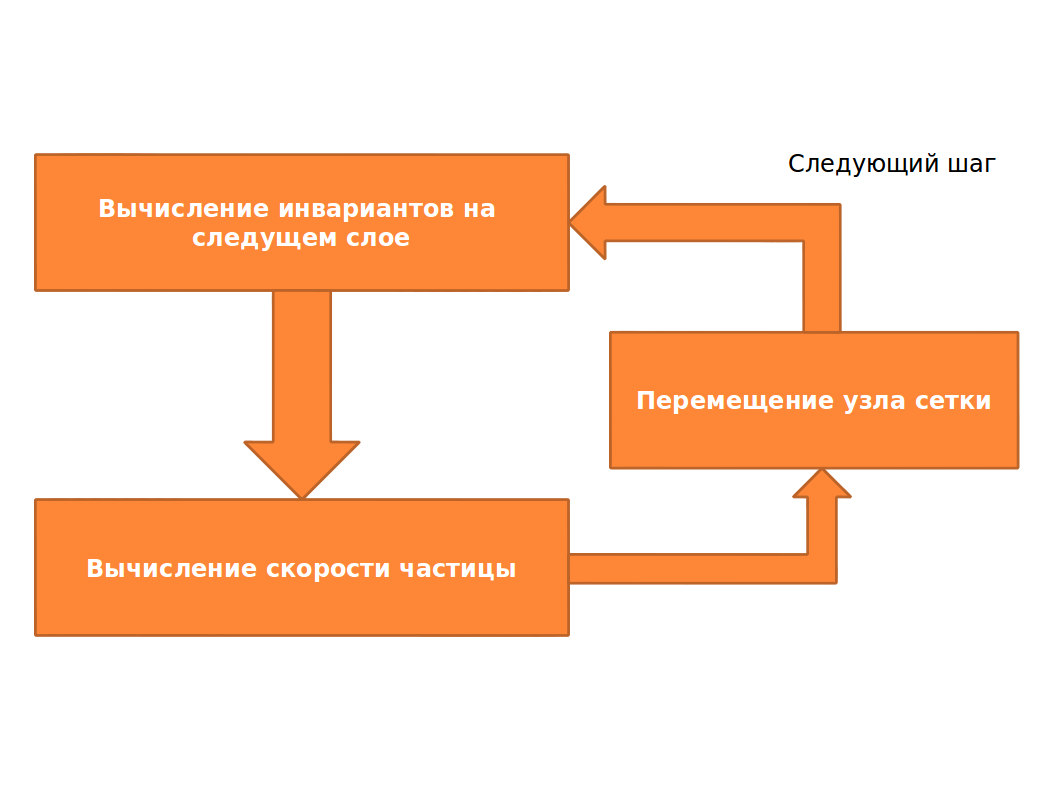
\includegraphics[width=1\linewidth]{png/1d/first-order.png}} a)
\end{minipage}
\begin{minipage}{0.47\linewidth}
\center{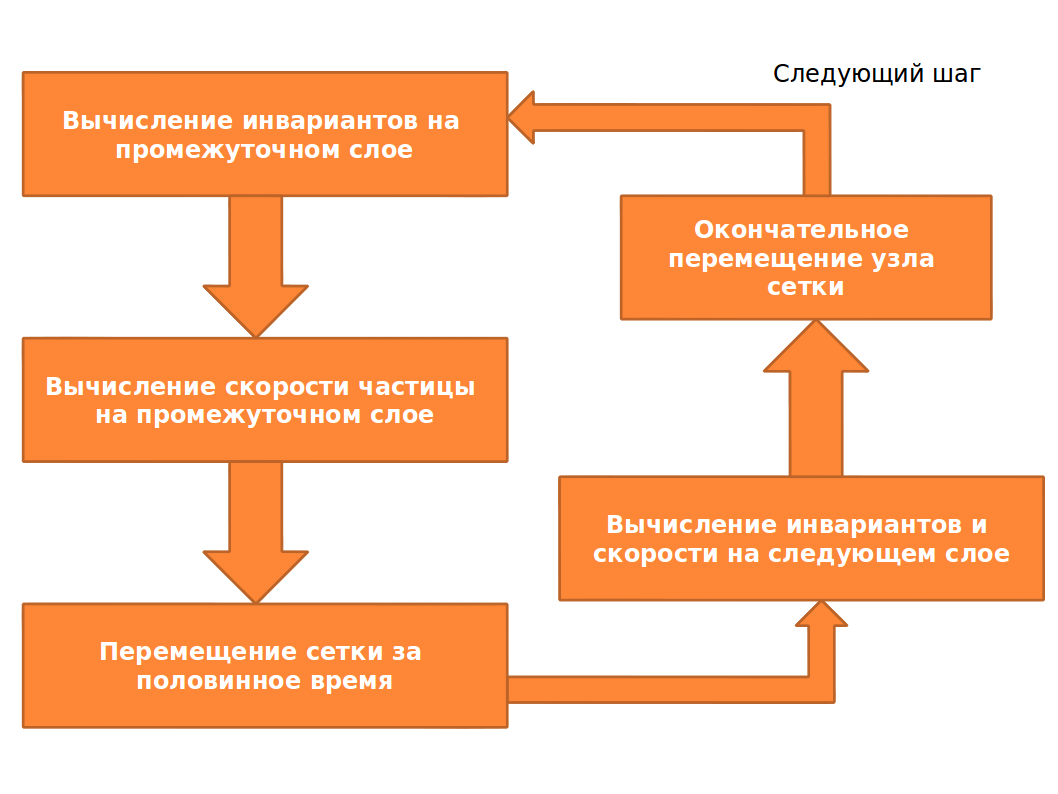
\includegraphics[width=1\linewidth]{png/1d/second-order.png}} b)
\end{minipage}
\caption{Схема расщепления на процессы распространения возмущения в веществе и переноса частиц вещества a) певого, b) второго порядка точности.}
\label{pic:splitting}
\end{figure} 

Далее рассмотрим идеи численного метода в трёхмерной постановке.
\subsection{Расщепление на упругую и пластическую части}
Пластическая задача решается расщеплением на два физических процесса: упругая деформация и пластическое течение. Расщепление проводилось на каждом из трёх подшагов по пространственным координатам, которые будут описаны ниже. На этапе предиктора расчёт значений на новом временном слое делается как для линейно-упругого тела. Затем, в случае выхода напряжений за пределы поверхности текучести, пластический корректор возвращает их обратно на $f(\sigma_{ij})=0$.
\subsection{Решение линейно-упругой части задачи}
\subsubsection{Матричная форма уравнений линейной упругости}
Уравнения \ref{rheology_equations} и \ref{tensor_qijkl} можно переписать в матричной
форме:
\begin{equation}
\label{matrix_equation}
\frac{\partial}{\partial{t}}\vec{u}+\mathbf{A}_x\frac{\partial}{\partial{x}}\vec{u}+
\mathbf{A}_y\frac{\partial}{\partial{y}}\vec{u}+
\mathbf{A}_z\frac{\partial}{\partial{z}}\vec{u}=\vec{f}.
\end{equation}
Здесь
$\vec{u}=\{v_x,v_y,v_z,\sigma_{xx},\sigma_{xy},\sigma_{xz},\sigma_{yy},\sigma_{yz},\sigma_{zz}\}^T$
-- вектор искомых функций, $\vec{f}$ -- вектор правых частей той же размерности,
$x,y,z$ --  независимые пространственные переменные, $t$ -- время,
\begin{displaymath}
\mathbf{A}_x =
\left( \begin{array}{cccccccccccc}
0 & 0 & 0 & -\frac 1 \rho & 0 & 0 & 0 & 0 & 0 \\ 
0 & 0 & 0 & 0 & -\frac 1 \rho & 0 & 0 & 0 & 0 \\ 
0 & 0 & 0 & 0 & 0 & -\frac 1 \rho & 0 & 0 & 0 \\ 
-\lambda-2\mu & 0 & 0 & 0 & 0 & 0 & 0 & 0 & 0 \\ 
0 & -\mu & 0 & 0 & 0 & 0 & 0 & 0 & 0 \\ 
0 & 0 & -\mu & 0 & 0 & 0 & 0 & 0 & 0 \\ 
-\lambda & 0 & 0 & 0 & 0 & 0 & 0 & 0 & 0 \\ 
0 & 0 & 0 & 0 & 0 & 0 & 0 & 0 & 0 \\ 
-\lambda & 0 & 0 & 0 & 0 & 0 & 0 & 0 & 0  
\end{array} \right),
\end{displaymath} 
\begin{displaymath}
\mathbf{A}_y =
\left( \begin{array}{cccccccccccc}
0 & 0 & 0 & 0 & -\frac 1 \rho & 0 & 0 & 0 & 0 \\ 
0 & 0 & 0 & 0 & 0 & 0 & -\frac 1 \rho & 0 & 0 \\ 
0 & 0 & 0 & 0 & 0 & 0 & 0 & -\frac 1 \rho & 0 \\ 
0 & -\lambda & 0 & 0 & 0 & 0 & 0 & 0 & 0 \\ 
-\mu & 0 & 0 & 0 & 0 & 0 & 0 & 0 & 0 \\ 
0 & 0 & 0 & 0 & 0 & 0 & 0 & 0 & 0 \\ 
0 & -\lambda-2\mu & 0 & 0 & 0 & 0 & 0 & 0 & 0 \\ 
0 & 0 & -\mu & 0 & 0 & 0 & 0 & 0 & 0 \\ 
0 & -\lambda & 0 & 0 & 0 & 0 & 0 & 0 & 0  
\end{array} \right),
\end{displaymath}
\begin{displaymath}
\mathbf{A}_z =
\left( \begin{array}{cccccccccccc}
0 & 0 & 0 & 0 & 0 & -\frac 1 \rho & 0 & 0 & 0 \\
0 & 0 & 0 & 0 & 0 & 0 & 0 & -\frac 1 \rho & 0 \\
0 & 0 & 0 & 0 & 0 & 0 & 0 & 0 & -\frac 1 \rho \\
0 & 0 & -\lambda & 0 & 0 & 0 & 0 & 0 & 0 \\
0 & 0 & 0 & 0 & 0 & 0 & 0 & 0 & 0 \\
-\mu & 0 & 0 & 0 & 0 & 0 & 0 & 0 & 0 \\
0 & 0 & -\lambda & 0 & 0 & 0 & 0 & 0 & 0 \\
0 & -\mu & 0 & 0 & 0 & 0 & 0 & 0 & 0 \\
0 & 0 & -(\lambda+2\mu) & 0 & 0 & 0 & 0 & 0 & 0
\end{array} \right).
\end{displaymath}
\subsubsection{Гиперболические свойства систем уравнений линейной упругости}
\label{hyperbolic}
Рассмотрим сначала одномерное уравнение вида
\begin{equation}
\frac{\partial}{\partial{t}}\vec{u}+\mathbf{A}\frac{\partial}{\partial{x}}\vec{u}=\vec{f}.
\label{advection_equation}
\end{equation}
Если матрица $\mathbf{A}$ имеет полный набор вещественных собственных значений, 
то такое уравнение называется гиперболическим, и его решения соответствуют 
процессам, которые носят волновой характер. В этом случае справедливо разложение:
$$\mathbf{A}=\mathbf\Omega^{-1}\mathbf\Lambda\mathbf\Omega,$$
где $\mathbf\Omega$ -- матрица, составленная из векторов ${\vec\omega_i}$, где
$\vec\omega_i$ есть собственные векторы матрицы $\mathbf A$,
удовлетворяющие соотношениям
$$\vec\omega_i\mathbf A=\lambda_i\vec\omega_i,$$
а $\mathbf\Lambda=diag\{\lambda_i\}$ -- диагональная матрица собственных
значений.
В предположении независимости компонент матрицы $\mathbf{A}$ от времени и координаты, домножив уравнение \ref{advection_equation} слева на $\Omega$, получаем
уравнение
$$\frac{\partial}{\partial t}\Omega{\vec u}+
\Lambda\frac{\partial}{\partial x}\Omega{\vec u}=\Omega{\vec f},$$
которое после перехода к Римановым инвариантам ${\vec v}=\Omega{\vec u}$
распадается на $n$ одномерных уравнений вида
\begin{equation}
\frac{\partial}{\partial t}{v_i}+\lambda_i\frac{\partial}{\partial
x}{v_i}={{\tilde f}_i},
\label{advection_equation_splitted}
\end{equation}
где ${{\tilde f}_i}=(\Omega{\vec f})_i$.
Таким образом, решение уравнения \ref{advection_equation} представляется в виде
суммы плоских волн, движущихся со скоростями $\lambda_i$. Вдоль прямой с наклоном 
$\frac{\partial x}{\partial t} = \lambda_i$, называемой характеристикой, \ref{advection_equation_splitted} переходит обыкновенное дифференциальное уравнение 
\begin{equation}
\frac{d{v_i}}{dt} = {{\tilde f}_i}.
\label{advection_equation_final} 
\end{equation}
Благодаря этому для численного решения \ref{advection_equation} предлагается использовать сеточно-характеристический метод, суть которого состоит в следующем. Из того узла $m$ временного слоя $n+1$, в котором требуется получить решение, опускаются характеристики.
\begin{figure}[h]
\center{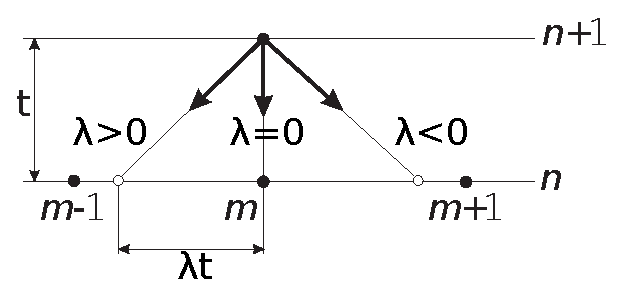
\includegraphics[width=0.5\textwidth]{eps/gcm-idea.eps}}
\caption{Принципиальная схема сеточно-характеристического метода.}
\end{figure}
Из точки пересечения характеристики со слоем $n$ значение $v_i$ переносится в 
точку $\xi^{n+1}_m$ путём решения \ref{advection_equation_final}:
$$v_i^{n+1}(\xi_m)=v^{n}_i(\xi_m-\lambda_i\tau) + {\tilde f}_i \tau.$$
Если характеристика не попадает точно в расcчётный узел, то применяются различные
методы реконструкции значения в данной точке (в данной работе используется
интерполяция соответствующего порядка).
\subsubsection{Расщепление по пространственным направлениям}				
Идея метода \cite{fedorenko} решения исходной задачи состоит в расщеплении по трём пространственным координатам, то есть в разделении на этапе численного решения трёхмерной системы уравнений \ref{matrix_equation} на три одномерных. На уровне дифференциальных операторов это может быть записано следующим образом:
\begin{equation}
\frac{\partial}{\partial t}\vec u+\mathbf{A}_x \frac{\partial}{\partial x}\vec u
= \vec f,
\label{matrix_equation_x}
\end{equation}
\begin{equation}
\frac{\partial}{\partial t}\vec u+\mathbf{A}_y \frac{\partial}{\partial y}\vec u
= \vec f,
\label{matrix_equation_y}
\end{equation}
\begin{equation}
\frac{\partial}{\partial t}\vec u+\mathbf{A}_z \frac{\partial}{\partial z}\vec u
= \vec f,
\label{matrix_equation_z}
\end{equation}
Эти уравнения решаются последовательно описанным в предыдущем параграфе методом с использованием
на очередном подшаге результатов, полученных на предыдущем подшаге.

\subsubsection{Расчёт граничных узлов}
Описанный выше чистый метод характеристик применяется только для расчёта внутренних узлов
сетки, то есть в том случае, если выпущенная из точки характеристика не
выходит за пределы области интегрирования. В противном случае для нахождения значений на новом временном слое  составляется система уравнений, в которой данные выводящих характеристик заменяются граничными и контактными условиями. Рассматриваемая система уравнений в граничных узлах имеет не более трёх
\cite{chelnokov} выводящих характеристик. 

Граничные условия могут быть нескольких видов, например (символы без волны -- для первого тела, с волной -- для второго):
\begin{itemize}
\item{жёстко закреплённая граница
\begin{eqnarray}
v_\tau=v_n=0; \nonumber
\end{eqnarray}}
\item{свободная граница
\begin{eqnarray}
\sigma_\tau=\sigma_n=0; \nonumber
\end{eqnarray}}
\item{скольжение тел друг относительно друга 
\begin{eqnarray}
v_n=\tilde{v}_n,\nonumber\\
\sigma_n=\tilde{\sigma}_n,\nonumber\\
\sigma_\tau=\tilde{\sigma}_\tau=0; \nonumber
\end{eqnarray}}
\item{слипание тел
\begin{eqnarray}
v_n=\tilde{v}_n,\nonumber\\
v_\tau=\tilde{v}_\tau.
\end{eqnarray}}
\end{itemize}
Эти условия доопределяют СЛАУ на значения инвариантов Римана на новом временном слое.

\subsection{Пластический корректор}
В данной работе был реализован простейший корректор, реализующий нормировку вектора напряжений. Этот способ известен как правило корректировки Уилкинса\cite{wilkins}, и верен только для идеальнопластической среды без упрочнения.

Рассчитанные в ходе эластичного предиктора напряжения в случае выхода за поверхность текучести  $f(\sigma_{ij}) \geq 0$ (см. \ref{mizes}), возвращаются на неё путём умножения на нормировочный коэффициент:
\begin{eqnarray}
s_{ij}^{n+1} = s_{ij}^e\frac{k_F}{J_2^e}	\\
J_2 = \sqrt{\frac{1}{2}s_{ij}s_{ij}}
\end{eqnarray} 
\clearpage
\newpage
\newpage
\section{Полученные результаты}
\subsection{Расчёты в }
\subsubsection{Линейная упругость}

\clearpage
\newpage
\section{Заключение}
Результаты, полученные в результате выполнения дипломного проекта:
\begin{itemize}
\item Рассмотрены различные подходы к описанию движения сплошной среды в сочетании с применяемыми к ним численными методами
\item Предложен метод моделирования сплошной среды в 1D с учётом движения и деформации тела, в том числе схема второго порядка точности по координате с учётом изменения характеристик среды в пространстве, точная со вторым порядком по времени схема расщепления рассчётного шага на движение рассчётной сетки и перенос возмущения
\item На основе данного метода реализован программный комплекс, моделирующий деформируемое твёрдое тело в случае одного пространственного измерения с поддержкой упругой и упругопластической реологии
\item Проведено сравнение результатов работы данного программного комплекса с результатами полуаналитического рассчёта на основе принципиально другого подхода к описанию сплошной среды и итерационного  метода. Получена сходимость результатов со вторым порядком точности по времени и координате
\item Предложен способ моделирования идеально-пластической реологии в 3D на основе правила корректировки Уилкинса
\item Данный способ реализован на основе существующего программного комплекса, поддерживающего линейную упругость в 3D
\item Проведено сравнение результатов. Получено удовольствие
\end{itemize}

\clearpage
\newpage
\begin{thebibliography}{99}
\addcontentsline{toc}{section}{Литература}
\bibitem{kukudganov}Кукуджанов В.Н. Вычислительная механика сплошное сред. - М.: Издательство 
Физико-математической литературы, 2008, с. 32, с. 242, с. 271.
\bibitem{resler}И.Реслер, Х.Хардерс, М.Бекер Механическое поведение конструкционных материалов. Перевод с немецкого. - Долгопрудный, Издательский дом <<Интеллект>>, 2011, с. 91-115
\bibitem{novatsky}Новацкий В. К. Теория упругости. — М. : Мир, 1975, c. 105-107.
\bibitem{sedov}Седов Л. И. Механика сплошной среды. Том 1. — М. : Наука, 1970, с. 143.
\bibitem{rebotnov}Работнов Ю.Н. Механика деформируемого твёрдого тела. — М.: Наука, 1988. — 712 с.
\bibitem{belocerkovsky}Белоцерковский О.М. Численное моделирование в механике
сплошных сред. — М.: Физико-математическая литература. 1994, 442 с.
\bibitem{magomedov}Магомедов К.М., Холодов А.С. Сеточно-характеристические
численные методы. — М.: Наука, 1988, 288 с.
\bibitem{holodov}Холодов А.С., Холодов Я.А. О критериях монотонности разностных
схем для уравнений гиперболического типа. 
\bibitem{chelnokov}Челноков Ф.Б. Численное моделирование деформационных
процессов в средах со сложной структурой.
\bibitem{fedorenko}Федоренко Р.П. Введение в вычислительную физику. М.:
Изд-во Моск. физ. -техн. ин-та, 1994, 528 с.
\bibitem{chushkin}Чушкин П.И. Метод характеристик для пространственных сверхзвуковых течений. –  Труды ВЦ АН СССР, 1968, c. 121.
\bibitem{petrov_chelnokov}Петров И.Б., Челноков Ф.Б. Численное исследование волновых процессов и процессов разрушения в многослойных преградах // Журнал вычислительной математики и математической физики – 2003, том 43, N 10, с. 1562-1579.
\bibitem{matyushev_petrov}Matyushev N.G., Petrov I.B. Mathematical Simulation of Deformation and Wave Processes in Multilayered Structures // Computational Mathematics and Mathematical Physics – 2009, Vol. 49, N 9, P. 1615-1621.
\bibitem{petrov_tormasov_holodov}Петров  И.Б., Тормасов А.Г., Холодов А.С. О численном изучении нестационарных процессов в деформируемых средах многослойной структуры // Механика твердого тела – 1989, N 4, с. 89-95.
\bibitem{golubev_kvasov_petrov}Голубев В.И., Квасов И.Е., Петров И.Б. Воздействие природных катастроф на наземные сооружения // Математическое моделирование – 2011, том 23, N 8, с. 46-54.
\bibitem{agapov_belocerkovsky_petrov}Агапов П.И., Белоцерковский О.М., Петров И.Б. Численное моделирование последствий механического воздействия на мозг человека при черепно-мозговой травме // Журнал вычислительной математики и математической физики – 2006, том 46, N 9, с. 1711-1720.
\bibitem{petrov}Петров И.Б. Волновые и откольные явления в слоистых оболочках конечной толщины // Механика твердого тела – 1986, N 4, с. 118-124.
\end{thebibliography}

\clearpage
\newpage
\section{Приложение}
\subsection{Диагонализация матриц из уравнений модели в случае орторомбической анизотропии и совпадения координатных осей с главными направлениями анизотропии}
\label{application1}

В указанном случае матрицы из уравнения \eqref{simple_matrix_equation} и их спектральное разложение $\mathbf{A} = \mathbf{\Omega}^{-1} \mathbf{L} \mathbf{\Omega}$ приведены ниже. Порядок собственных значений в $\mathbf{L}$ и, соответственно, собственных векторов в $\mathbf{\Omega}^{-1}$ следующий: поперечная волна против оси, поперечная волна вдоль оси, другая поперечная волна против оси, другая поперечная волна вдоль оси, продольная волна против оси, продольная волна вдоль оси, три неподвижных инварианта.

\[\mathbf{A}_x = \\
\begin{pmatrix}0 & 0 & 0 & -\frac{1}{\rho} & 0 & 0 & 0 & 0 & 0\cr 0 & 0 & 0 & 0 & -\frac{1}{\rho} & 0 & 0 & 0 & 0\cr 0 & 0 & 0 & 0 & 0 & -\frac{1}{\rho} & 0 & 0 & 0\cr -c_{11} & 0 & 0 & 0 & 0 & 0 & 0 & 0 & 0\cr 0 & -c_{66} & 0 & 0 & 0 & 0 & 0 & 0 & 0\cr 0 & 0 & -c_{55} & 0 & 0 & 0 & 0 & 0 & 0\cr -c_{12} & 0 & 0 & 0 & 0 & 0 & 0 & 0 & 0\cr 0 & 0 & 0 & 0 & 0 & 0 & 0 & 0 & 0\cr -c_{13} & 0 & 0 & 0 & 0 & 0 & 0 & 0 & 0\end{pmatrix}\]

\[\mathbf{L}_x = \\
diag(-\sqrt{\frac{c_{66}}{\rho}},\sqrt{\frac{c_{66}}{\rho}},-\sqrt{\frac{c_{55}}{\rho}},\sqrt{\frac{c_{55}}{\rho}},-\sqrt{\frac{c_{11}}{\rho}},\sqrt{\frac{c_{11}}{\rho}},0,0,0)\]

\[{\mathbf{\Omega}_x}^{-1} = 
\begin{pmatrix}0 & 0 & 0 & 0 & \frac{1}{2} & \frac{1}{2} & 0 & 0 & 0\cr \frac{1}{2} & \frac{1}{2} & 0 & 0 & 0 & 0 & 0 & 0 & 0\cr 0 & 0 & \frac{1}{2} & \frac{1}{2} & 0 & 0 & 0 & 0 & 0\cr 0 & 0 & 0 & 0 & \frac{1}{2}\,\sqrt{c_{11} \rho} & -\frac{1}{2}\,\sqrt{c_{11} \rho} & 0 & 0 & 0\cr \frac{1}{2}\,\sqrt{c_{66} \rho} & -\frac{1}{2}\,\sqrt{c_{66} \rho} & 0 & 0 & 0 & 0 & 0 & 0 & 0\cr 0 & 0 & \frac{1}{2}\,\sqrt{c_{55} \rho} & -\frac{1}{2}\,\sqrt{c_{55} \rho} & 0 & 0 & 0 & 0 & 0\cr 0 & 0 & 0 & 0 & \frac{\frac{1}{2}\,c_{12}\,\sqrt{\rho}}{\sqrt{c_{11}}} & -\frac{\frac{1}{2}\,c_{12}\,\sqrt{\rho}}{\sqrt{c_{11}}} & 1 & 0 & 0\cr 0 & 0 & 0 & 0 & 0 & 0 & 0 & 1 & 0\cr 0 & 0 & 0 & 0 & \frac{\frac{1}{2}\,c_{13}\,\sqrt{\rho}}{\sqrt{c_{11}}} & -\frac{\frac{1}{2}\,c_{13}\,\sqrt{\rho}}{\sqrt{c_{11}}} & 0 & 0 & 1\end{pmatrix}\]

\[\mathbf{\Omega}_x = \\
\begin{pmatrix}0 & 1 & 0 & 0 & \frac{1}{\sqrt{c_{66} \rho}} & 0 & 0 & 0 & 0\cr 0 & 1 & 0 & 0 & -\frac{1}{\sqrt{c_{66} \rho}} & 0 & 0 & 0 & 0\cr 0 & 0 & 1 & 0 & 0 & \frac{1}{\sqrt{c_{55} \rho}} & 0 & 0 & 0\cr 0 & 0 & 1 & 0 & 0 & -\frac{1}{\sqrt{c_{55} \rho}} & 0 & 0 & 0\cr 1 & 0 & 0 & \frac{1}{\sqrt{c_{11} \rho}} & 0 & 0 & 0 & 0 & 0\cr 1 & 0 & 0 & -\frac{1}{\sqrt{c_{11} \rho}} & 0 & 0 & 0 & 0 & 0\cr 0 & 0 & 0 & -\frac{c_{12}}{c_{11}} & 0 & 0 & 1 & 0 & 0\cr 0 & 0 & 0 & 0 & 0 & 0 & 0 & 1 & 0\cr 0 & 0 & 0 & -\frac{c_{13}}{c_{11}} & 0 & 0 & 0 & 0 & 1\end{pmatrix}\]


\[\mathbf{A}_y = \\
\begin{pmatrix}0 & 0 & 0 & 0 & -\frac{1}{\rho} & 0 & 0 & 0 & 0\cr 0 & 0 & 0 & 0 & 0 & 0 & -\frac{1}{\rho} & 0 & 0\cr 0 & 0 & 0 & 0 & 0 & 0 & 0 & -\frac{1}{\rho} & 0\cr 0 & -c_{12} & 0 & 0 & 0 & 0 & 0 & 0 & 0\cr -c_{66} & 0 & 0 & 0 & 0 & 0 & 0 & 0 & 0\cr 0 & 0 & 0 & 0 & 0 & 0 & 0 & 0 & 0\cr 0 & -c_{22} & 0 & 0 & 0 & 0 & 0 & 0 & 0\cr 0 & 0 & -c_{44} & 0 & 0 & 0 & 0 & 0 & 0\cr 0 & -c_{23} & 0 & 0 & 0 & 0 & 0 & 0 & 0\end{pmatrix}\]


\[\mathbf{L}_y = \\
(-\sqrt{\frac{c_{66}}{\rho}},\sqrt{\frac{c_{66}}{\rho}},-\sqrt{\frac{c_{44}}{\rho}},\sqrt{\frac{c_{44}}{\rho}},-\sqrt{\frac{c_{22}}{\rho}},\sqrt{\frac{c_{22}}{\rho}}, 0, 0, 0)\]


\[{\mathbf{\Omega}_y}^{-1} = 
\begin{pmatrix}\frac{1}{2} & \frac{1}{2} & 0 & 0 & 0 & 0 & 0 & 0 & 0\cr 0 & 0 & 0 & 0 & \frac{1}{2} & \frac{1}{2} & 0 & 0 & 0\cr 0 & 0 & \frac{1}{2} & \frac{1}{2} & 0 & 0 & 0 & 0 & 0\cr 0 & 0 & 0 & 0 & \frac{\frac{1}{2}\,c_{12}}{\sqrt{\frac{c_{22}}{\rho}}} & -\frac{\frac{1}{2}\,c_{12}}{\sqrt{\frac{c_{22}}{\rho}}} & 1 & 0 & 0\cr \frac{1}{2}\,\sqrt{c_{66} \rho} & -\frac{1}{2}\,\sqrt{c_{66} \rho} & 0 & 0 & 0 & 0 & 0 & 0 & 0\cr 0 & 0 & 0 & 0 & 0 & 0 & 0 & 1 & 0\cr 0 & 0 & 0 & 0 & \frac{1}{2}\,\sqrt{c_{22} \rho} & -\frac{1}{2}\,\sqrt{c_{22} \rho} & 0 & 0 & 0\cr 0 & 0 & \frac{1}{2}\,\sqrt{c_{44} \rho} & -\frac{1}{2}\,\sqrt{c_{44} \rho} & 0 & 0 & 0 & 0 & 0\cr 0 & 0 & 0 & 0 & \frac{\frac{1}{2}\,c_{23}\,\sqrt{\rho}}{\sqrt{c_{22}}} & -\frac{\frac{1}{2}\,c_{23}\,\sqrt{\rho}}{\sqrt{c_{22}}} & 0 & 0 & 1\end{pmatrix}\]

\[\mathbf{\Omega}_y = \\
\begin{pmatrix}1 & 0 & 0 & 0 & \frac{1}{\sqrt{c_{66} \rho}} & 0 & 0 & 0 & 0\cr 1 & 0 & 0 & 0 & -\frac{1}{\sqrt{c_{66} \rho}} & 0 & 0 & 0 & 0\cr 0 & 0 & 1 & 0 & 0 & 0 & 0 & \frac{1}{\sqrt{c_{44} \rho}} & 0\cr 0 & 0 & 1 & 0 & 0 & 0 & 0 & -\frac{1}{\sqrt{c_{44} \rho}} & 0\cr 0 & 1 & 0 & 0 & 0 & 0 & \frac{1}{\sqrt{c_{22} \rho}} & 0 & 0\cr 0 & 1 & 0 & 0 & 0 & 0 & -\frac{1}{\sqrt{c_{22} \rho}} & 0 & 0\cr 0 & 0 & 0 & 1 & 0 & 0 & -\frac{c_{12}}{c_{22}} & 0 & 0\cr 0 & 0 & 0 & 0 & 0 & 1 & 0 & 0 & 0\cr 0 & 0 & 0 & 0 & 0 & 0 & -\frac{c_{23}}{c_{22}} & 0 & 1\end{pmatrix}\]


\[\mathbf{A}_z = \\
\begin{pmatrix}0 & 0 & 0 & 0 & 0 & -\frac{1}{\rho} & 0 & 0 & 0\cr 0 & 0 & 0 & 0 & 0 & 0 & 0 & -\frac{1}{\rho} & 0\cr 0 & 0 & 0 & 0 & 0 & 0 & 0 & 0 & -\frac{1}{\rho}\cr 0 & 0 & -c_{13} & 0 & 0 & 0 & 0 & 0 & 0\cr 0 & 0 & 0 & 0 & 0 & 0 & 0 & 0 & 0\cr -c_{55} & 0 & 0 & 0 & 0 & 0 & 0 & 0 & 0\cr 0 & 0 & -c_{23} & 0 & 0 & 0 & 0 & 0 & 0\cr 0 & -c_{44} & 0 & 0 & 0 & 0 & 0 & 0 & 0\cr 0 & 0 & -c_{33} & 0 & 0 & 0 & 0 & 0 & 0\end{pmatrix}\]

\[\mathbf{L}_z = \\
(-\sqrt{\frac{c_{55}}{\rho}},\sqrt{\frac{c_{55}}{\rho}},-\sqrt{\frac{c_{44}}{\rho}},\sqrt{\frac{c_{44}}{\rho}},-\sqrt{\frac{c_{33}}{\rho}},\sqrt{\frac{c_{33}}{\rho}},0, 0, 0)\]

\[{\mathbf{\Omega}_z}^{-1} = 
\begin{pmatrix}\frac{1}{2} & \frac{1}{2} & 0 & 0 & 0 & 0 & 0 & 0 & 0\cr 0 & 0 & \frac{1}{2} & \frac{1}{2} & 0 & 0 & 0 & 0 & 0\cr 0 & 0 & 0 & 0 & \frac{1}{2} & \frac{1}{2} & 0 & 0 & 0\cr 0 & 0 & 0 & 0 & \frac{\frac{1}{2}\,c_{13}\,\sqrt{\rho}}{\sqrt{c_{33}}} & -\frac{\frac{1}{2}\,c_{13}\,\sqrt{\rho}}{\sqrt{c_{33}}} & 1 & 0 & 0\cr 0 & 0 & 0 & 0 & 0 & 0 & 0 & 1 & 0\cr \frac{1}{2}\,\sqrt{c_{55} \rho} & -\frac{1}{2}\,\sqrt{c_{55} \rho} & 0 & 0 & 0 & 0 & 0 & 0 & 0\cr 0 & 0 & 0 & 0 & \frac{\frac{1}{2}\,c_{23}\,\sqrt{\rho}}{\sqrt{c_{33}}} & -\frac{\frac{1}{2}\,c_{23}\,\sqrt{\rho}}{\sqrt{c_{33}}} & 0 & 0 & 1\cr 0 & 0 & \frac{1}{2}\,\sqrt{c_{44} \rho} & -\frac{1}{2}\,\sqrt{c_{44} \rho} & 0 & 0 & 0 & 0 & 0\cr 0 & 0 & 0 & 0 & \frac{1}{2}\,\sqrt{c_{33} \rho} & -\frac{1}{2}\,\sqrt{c_{33} \rho} & 0 & 0 & 0\end{pmatrix}\]

\[\mathbf{\Omega}_z = \\
\begin{pmatrix}1 & 0 & 0 & 0 & 0 & \frac{1}{\sqrt{c_{55} \rho}} & 0 & 0 & 0\cr 1 & 0 & 0 & 0 & 0 & -\frac{1}{\sqrt{c_{55} \rho}} & 0 & 0 & 0\cr 0 & 1 & 0 & 0 & 0 & 0 & 0 & \frac{1}{\sqrt{c_{44} \rho}} & 0\cr 0 & 1 & 0 & 0 & 0 & 0 & 0 & -\frac{1}{\sqrt{c_{44} \rho}} & 0\cr 0 & 0 & 1 & 0 & 0 & 0 & 0 & 0 & \frac{1}{\sqrt{c_{33} \rho}}\cr 0 & 0 & 1 & 0 & 0 & 0 & 0 & 0 & -\frac{1}{\sqrt{c_{33} \rho}}\cr 0 & 0 & 0 & 1 & 0 & 0 & 0 & 0 & -\frac{1\,c_{13}}{c_{33}}\cr 0 & 0 & 0 & 0 & 1 & 0 & 0 & 0 & 0\cr 0 & 0 & 0 & 0 & 0 & 0 & 1 & 0 & -\frac{c_{23}}{c_{33}}\end{pmatrix}\]




\end{document}



